{%%%%%%%%%%%%%%%%%%%%%%%%%
%% SITE A GARDER : 
%% http://titilog.free.fr/




\documentclass{beamer}
  %\usepackage[version=3]{mhchem}
\usepackage{caption}
\usepackage[french]{babel}
\captionsetup[figure]{labelformat=empty}
  \usetheme{m} %
  \usepackage{fontspec}
  \usepackage{biblatex}
\bibliography{geodis}
  \usefonttheme[onlymath]{serif} 
  \usepackage{amsmath}
  \usepackage{subcaption}
  \title{Estimation de plans orthogonaux sur des volumes tubulaires }
  \author{\textbf{F. \textsc{Grélard}}\inst{1}, F. \textsc{Baldacci}\inst{1}, A.  \textsc{Vialard}\inst{1} et J.-O.  \textsc{Lachaud}\inst{2}}
  \institute{1. Univ. Bordeaux, LaBRI,
  \and 2. Université Savoie Mont Blanc, LAMA}
  \titlegraphic{
  
\includegraphics[width=0.1875\textwidth]{fig/new-logo-labri}~\hspace*{0.0625\textwidth}~%
  
\includegraphics[width=0.1875\textwidth]{fig/univ_bordeaux}\hspace*{0.0625\textwidth}~%
  
\includegraphics[width=0.1875\textwidth]{fig/Logo-Lama-USMB}\hspace*{0.0625\textwidth}~%
  
\includegraphics[width=0.1875\textwidth]{fig/logo_uds}\hspace*{0.0625\textwidth}~%
}
  
  
\let\oldfootnotesize\footnotesize
\renewcommand*{\footnotesize}{\oldfootnotesize\tiny}
\newrobustcmd*{\footlessfullcite}{\AtNextCite{\renewbibmacro{in:}{}\renewbibmacro{year:}{}}\footfullcite}
\newrobustcmd*{\lessfullcite}{\AtNextCite{\renewbibmacro{in:}{}\renewbibmacro{year:}{}}\fullcite}

%http://mcclinews.free.fr/latex/introbeamer/les_couleurs.html
  \begin{document}
%affiche le logo en bas à droite
\logo{
\includegraphics[height=0.5cm]{fig/logo-labri.png}}
% enlève la barre de navigation
\setbeamertemplate{navigation symbols}{
}
\setbeamertemplate{blocks}[rounded][shadow=true]
% Ombre aux blocks
\setbeamertemplate{caption}{\insertcaption}


\date{GT GeoDis, 25 novembre 2015}  % set the Date
\AtBeginSection[]{
	\begin{frame}[plain]{Sommaire}
		\tableofcontents[currentsection, hideothersubsections]
	\end{frame}
}
\renewcommand{\insertnavigation}[1]{}

\begin{frame}[plain]
	\titlepage
\end{frame}


\section{Introduction}
\begin{frame}
	\frametitle{Contexte}
	\vspace{-0.2cm}
				
			\begin{block}{Contexte}
				\begin{itemize}
					\item Acquisition $\Rightarrow$ segmentation
					\item Volumes discrets tubulaires (bronches, vaisseaux sanguins, neurones)
					\item Besoin de mesures et de caractérisations
				\end{itemize}
			\end{block}
					
			\begin{figure}
				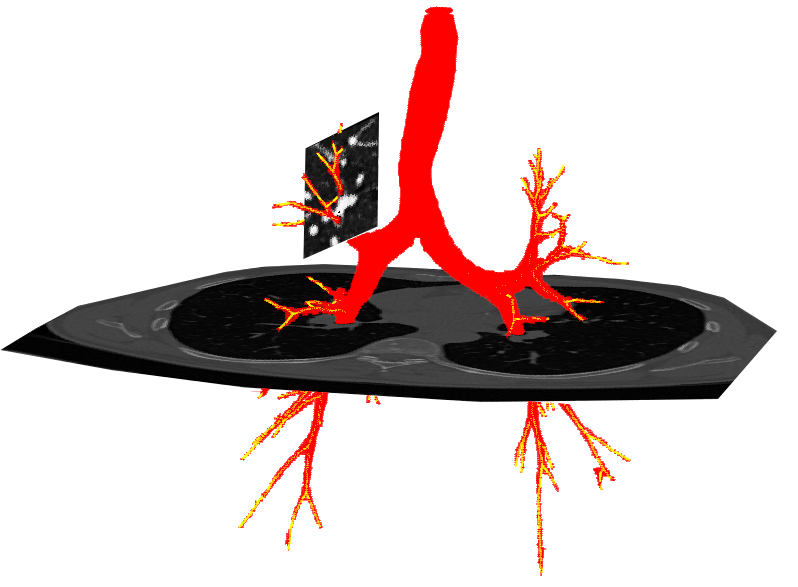
\includegraphics[scale=0.2]{fig/bronche.png}
			\end{figure}

\end{frame}

\begin{frame}
	\begin{columns}
		\begin{column}[t]{4cm}
			\frametitle{Plan orthogonal}
										
			\begin{block}{Applications}
				Profils sur l'ensemble du tube:
				\begin{itemize}
					\item De diamètre
					\item D'aire
					\item D'ellipticité
					\item D'épaisseur de paroi
				\end{itemize}
			\end{block}
		\end{column}
							
		\begin{column}[t]{6cm}
		\vspace{-0.4cm}
			\begin{figure}
				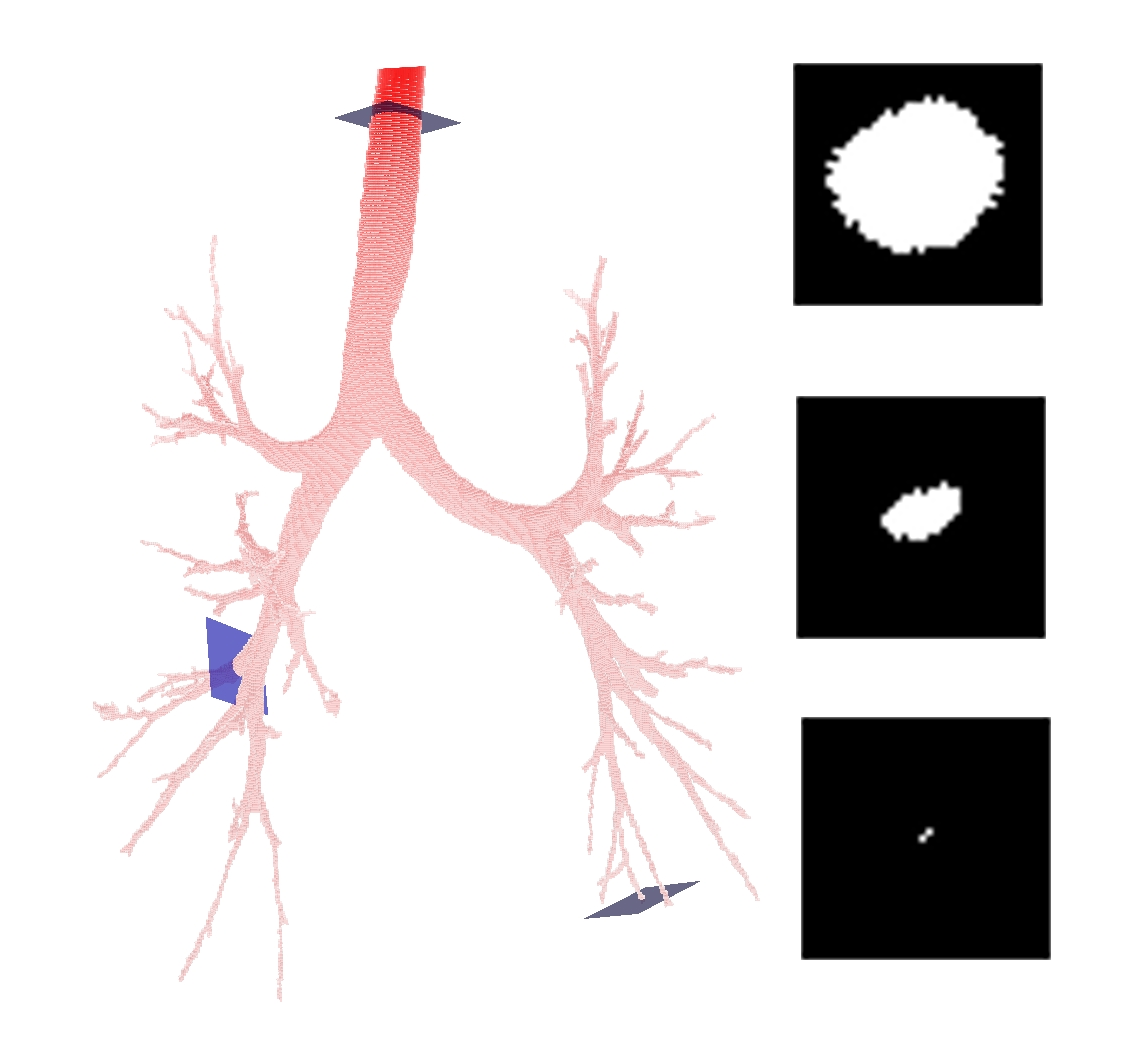
\includegraphics[width=\textwidth]{fig/skeletonPlane.png}
				\caption{Plans orthogonaux (en bleu) et sections avec le volume (à droite)}
			\end{figure}
		\end{column}
	\end{columns}
\end{frame}

\section{Travaux précédents}
\begin{frame}
	\frametitle{Principe général}

	\begin{columns}
		\begin{column}[t]{5cm}
			Etapes de l'algorithme:
			\begin{enumerate}
				\item<1,2,3> Calcul du squelette curviligne
				\item<2,3> Estimation de la tangente en chaque point du squelette
				\item<3> Pour tout point, la normale du plan orthogonal correspond à la tangente.
			\end{enumerate}
		\end{column}
								
		\begin{column}[t]{6cm}
			\begin{figure}
				\includegraphics<1>[width=\textwidth]{fig/closeup.jpg.png}
				\includegraphics<2>[width=\textwidth]{fig/closeuptang.jpg.png}
				\includegraphics<3>[width=\textwidth]{fig/vcmfullcloseup.jpg.png}
			\end{figure}
		\end{column}
	\end{columns}
				
\end{frame}






\begin{frame}
	\frametitle{Tangentes 3D}
	\vspace{-0.5cm}
	$\lambda$-MST: estimateur de tangentes à une courbe discrète 2D \footlessfullcite{lachaudfast2007} et 3D \footlessfullcite{postolski2012tangent}. \\
						
	$\Rightarrow$ Tangente en un point : moyenne pondérée des vecteurs directeurs des segments maximaux passant par ce point.
	\vspace{-0.4cm}
	\begin{columns}[b]
		\begin{column}{0.48\textwidth}
			\begin{figure}
				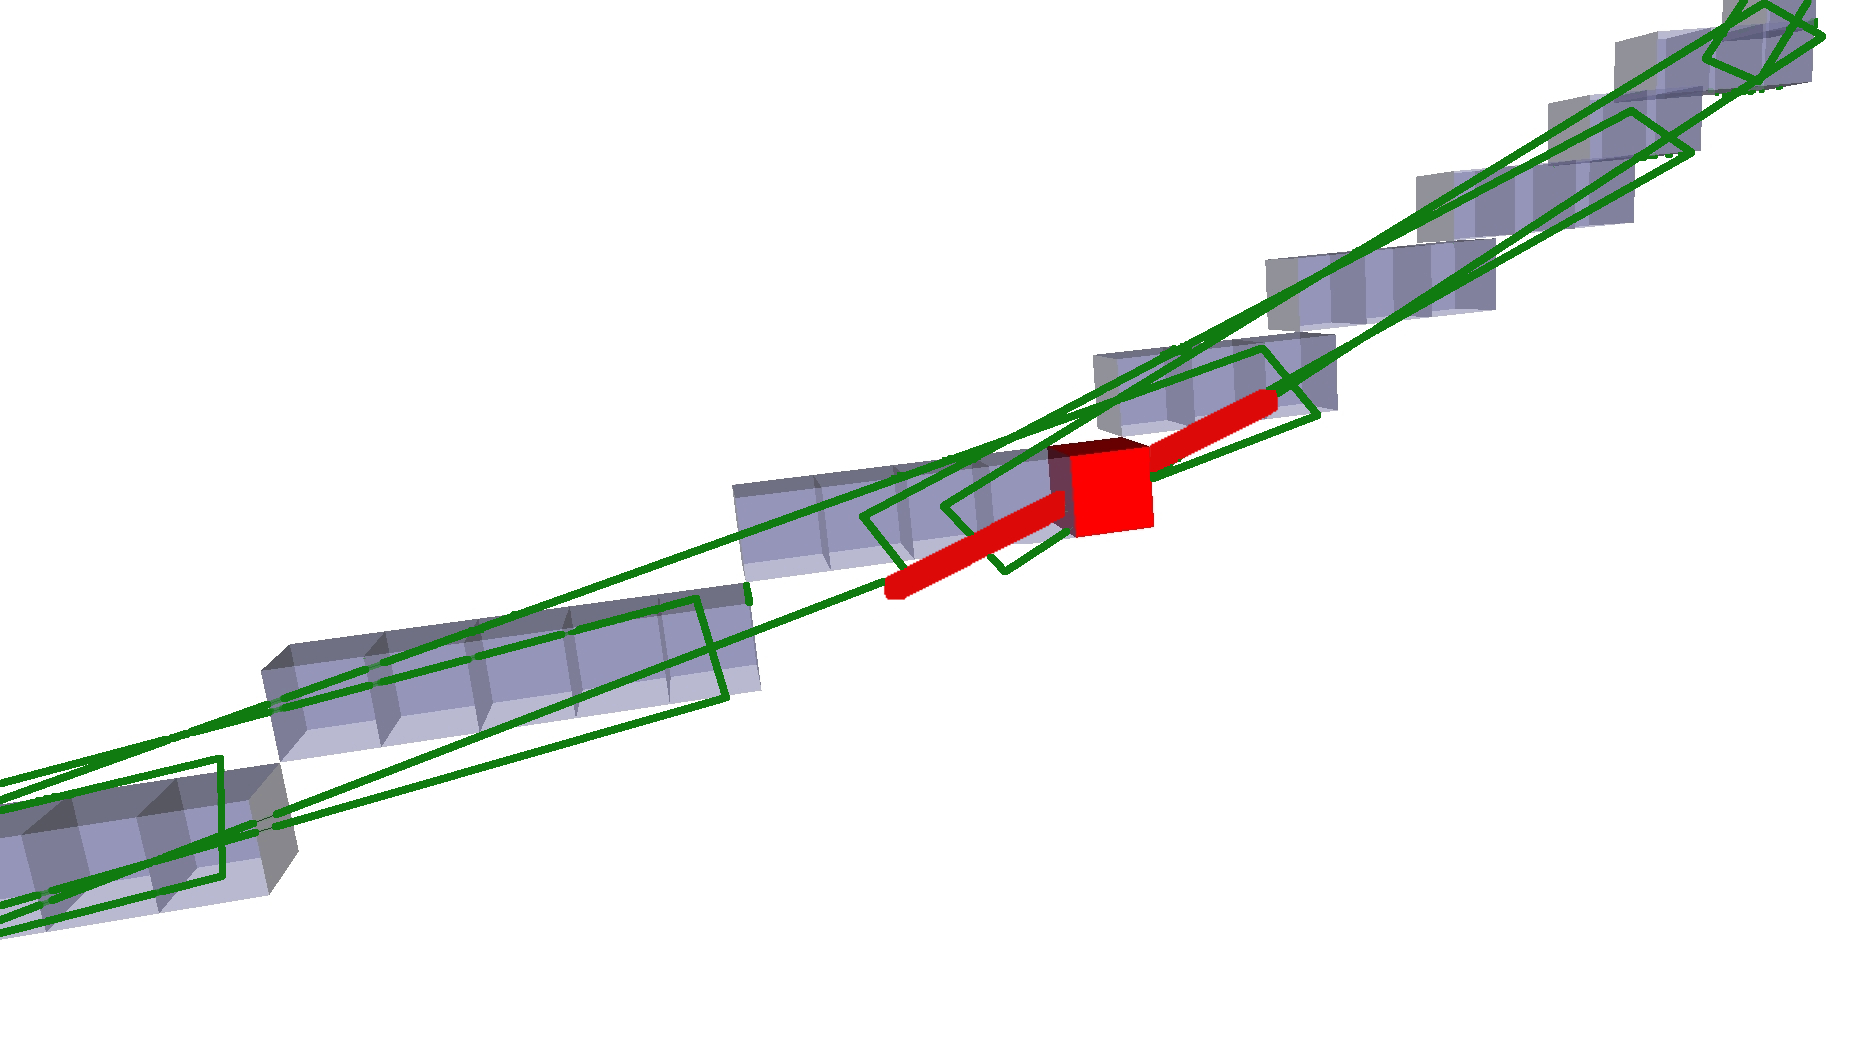
\includegraphics[width=0.9\textwidth]{fig/tangent3D2.png}
				\caption{Segments de droite maximaux (en vert) et tangente (en rouge)}
			\end{figure}
		\end{column}
											
		\begin{column}{0.48\textwidth}
			\begin{figure}
				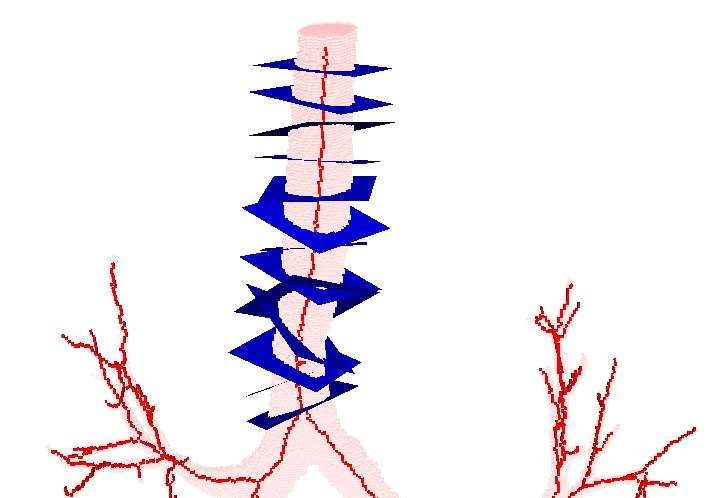
\includegraphics[width=0.9\textwidth]{fig/mst13closeup.png}
				\caption{Sensibilité aux irrégularités du squelette}
			\end{figure}
		\end{column}
	\end{columns}
						
						
							
\end{frame}



\section{Estimation de plans orthogonaux par les VCM}
\begin{frame}
	\frametitle{Voronoï Covariance Measure (VCM)}
			
	\begin{block}{VCM\footnotemark}
			La cellule de Voronoï est allongée
			dans le sens de la normale à la surface.
	\end{block}\footnotetext{\lessfullcite{Alliez}}
			
	\begin{figure}																
				\centering
				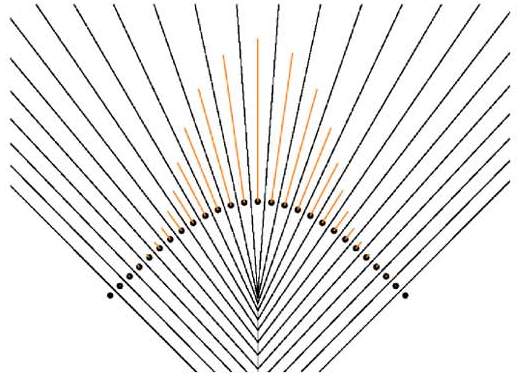
\includegraphics[width=0.4\textwidth]{fig/continuousvoronoi.png}
		\caption{Relation entre normales (en orange) et les cellules de Voronoï \footlessfullcite{merigot_vcm}.}
	\end{figure}
	\vspace{-0.3cm}
			
\end{frame}

\begin{frame}
	\frametitle{VCM discret}
	\vspace{-0.5cm}
		\begin{figure}
		\includegraphics<1>[scale=0.33]{fig/dvcm-r6.png}
		\includegraphics<2>[scale=0.33]{fig/dvcm-r5.png}
		\includegraphics<3>[scale=0.33]{fig/dvcm-r4.png}
		\includegraphics<4>[scale=0.33]{fig/dvcm-r3.png}
		\includegraphics<5>[scale=0.33]{fig/dvcm-r8.png}
		\includegraphics<6>[scale=0.33]{fig/dvcm-r7.png}
	\end{figure}
	\vspace{-0.6cm}
	\begin{itemize}
		\item<2,3,4,5,6> L'offset de $O$ de rayon $R$ est $O^R=\cup_{o \in O} B(o, R)$ 
		\item<3,4,5,6> $y$ : point où l'on veut mesurer le VCM
		\item<4,5,6> $X$ : $B(y,r) \cap O$
		\item<5,6> $\text{Vor}(x)$ : la cellule de Voronoï de $x \in X$ 
		\item<5,6> $p_O(x)$ : site de la cellule de Voronoï de $x$
		\item<6> Domaine d'intégration : $DI_O(y, r, R) = \cup_{x \in X}\ (\text{Vor}(x) \cap O^R)$
	\end{itemize}
					

			
\end{frame}

\begin{frame}
	\frametitle{VCM discret}
	\begin{block}{Mesure de covariance}
	\begin{itemize}
		\item Le VCM est donné par: 		
		\[
			\mathcal{V}_O(y,r,R) = \sum_{x^{‎\prime} \in DI_O(y,r,R)} (x^{‎\prime} - p_O(x^{‎\prime}))(x^{‎\prime}-p_O(x^{‎\prime}))^t
		\]
		\item Normale = vecteur avec la plus grande valeur propre.
	\end{itemize}
	\end{block}
	\begin{block}{Propriétés\footnotemark}
		\begin{itemize}
			\item Convergence asymptotique
			\item Robuste au bruit Hausdorff, aux outliers
		\end{itemize}
	\end{block}\footnotetext{\lessfullcite{CuelDB14}}
	\vspace{0.5cm}
							
	
\end{frame}

\begin{frame}
	\frametitle{A partir du squelette}
	\begin{itemize}
		\item VCM appliqué à une courbe 3D (squelette)
		\item Cellule de Voronoï allongée dans deux directions: définissent la base du plan orthogonal\footlessfullcite{Grelard}.
		\item Domaine d'intégration: utilisation des connaissances a priori (rayon du tube)
	\end{itemize}
	
	\vspace{-0.5cm}	
	\begin{figure}				
		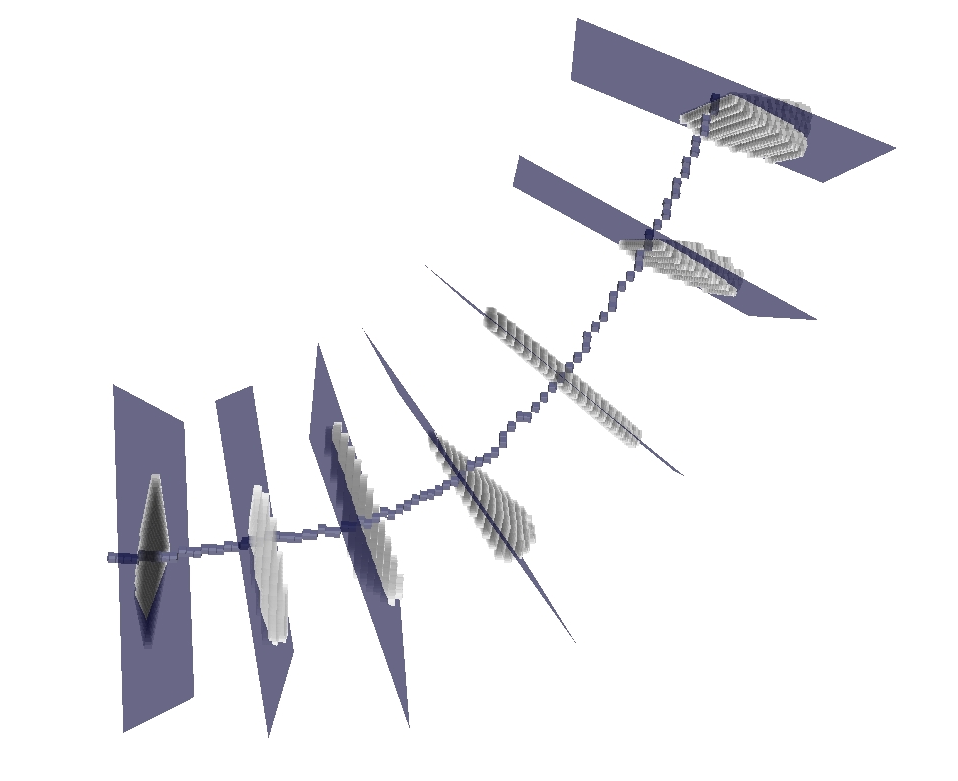
\includegraphics[clip, trim=0 3cm 0 0, scale=0.16]{fig/vcm_courbe.png}
		\caption{Cellules de Voronoï et lien avec plans orthogonaux}
	\end{figure}
		
\end{frame}

\begin{frame}
	\frametitle{A partir du volume}
	\begin{itemize}
		
		\item Dans le volume: $\text{Vor}(x) = x$.
		\item Plan orthogonal = somme des contributions des cellules de Voronoï en surface.
		\item Problème: paramétrer le domaine d'intégration ($r$)
	\end{itemize}
	\begin{figure}
		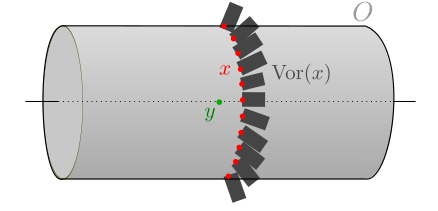
\includegraphics[clip, trim=0 0cm 0 3 cm, scale=0.35]{fig/cylindercone.png}
		\caption{Cellules de Voronoï $\text{Vor}(x)$ et plan orthogonal}
	\end{figure}
\end{frame}

\section{Résultats}
\begin{frame}
	\frametitle{Volume synthétique (1)}
	
		
			\begin{itemize}
				\item Volume tubulaire avec des perturbations en surface 
				\item Mesures quantitatives sur les sections obtenues dans le volume (aire et rotondité)
				\item Comparaison avec $\lambda$-MST
			\end{itemize}
				
			\begin{figure}[H]
				\centering
				\begin{subfigure}[t]{0.45\textwidth}
					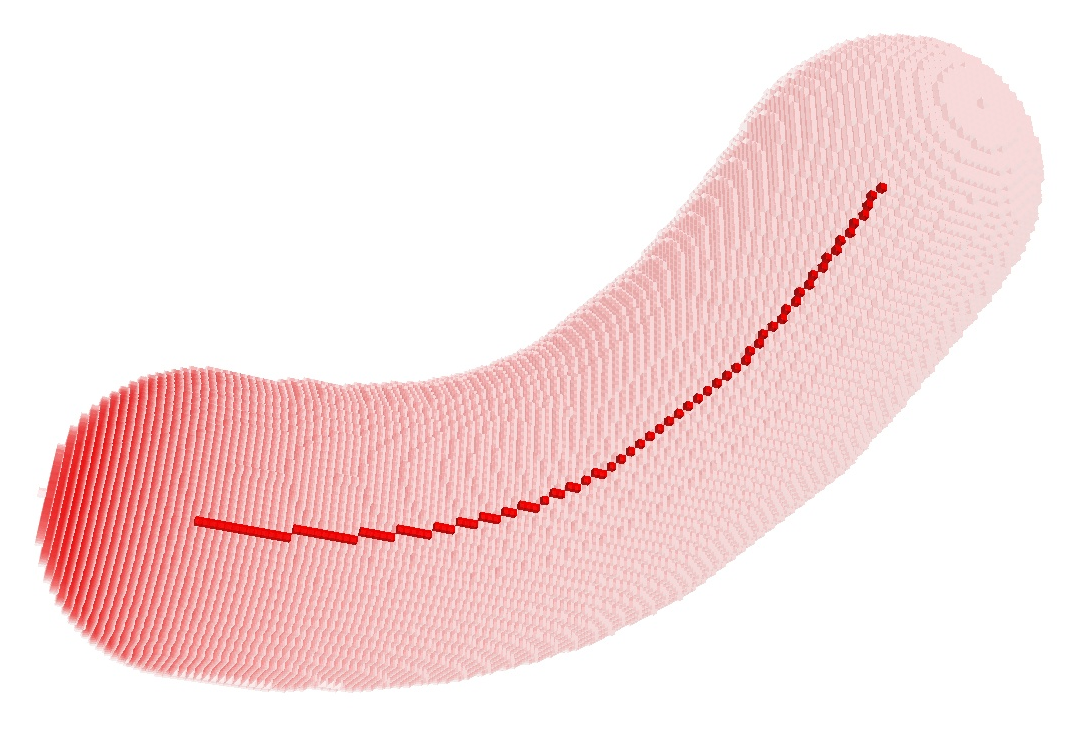
\includegraphics[width=\textwidth]{fig/boudin.png}
					\caption{}
					\label{fig:boudinnoisy}
				\end{subfigure}%
				\begin{subfigure}[t]{0.45\textwidth}
					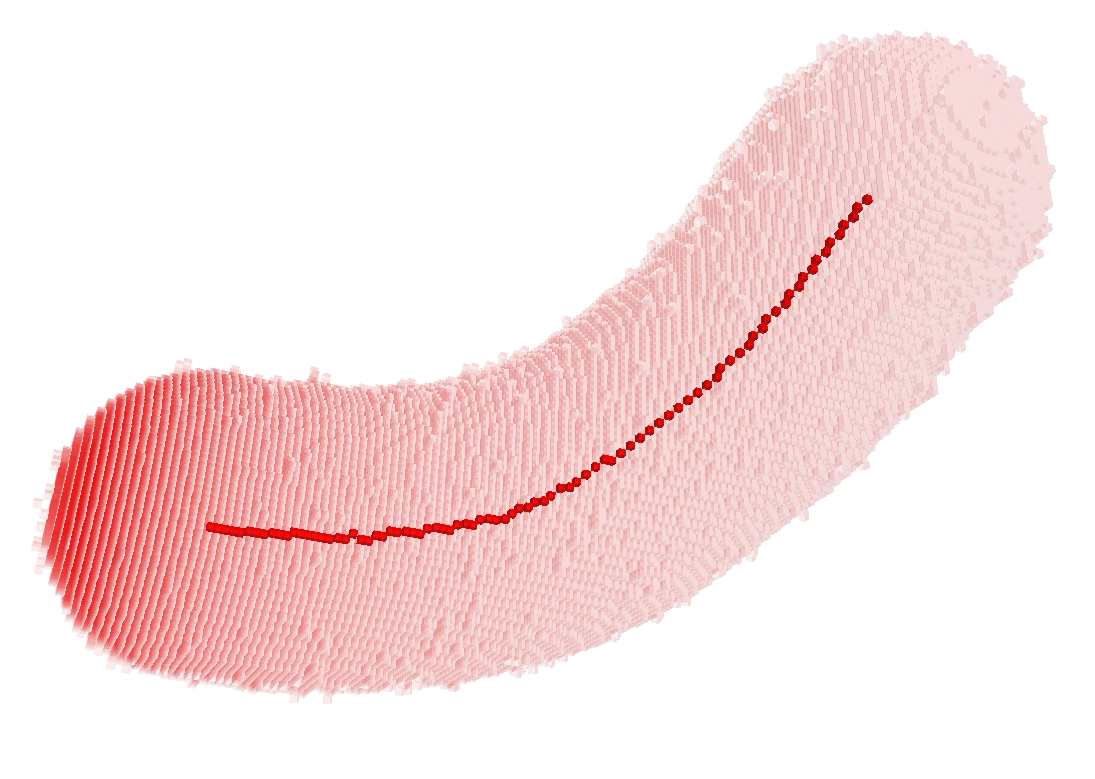
\includegraphics[width=\textwidth]{fig/boudinbruite.png}
					\caption{}
					\label{fig:thskeleton}
				\end{subfigure}
			\end{figure}		
\end{frame}

\begin{frame}
\frametitle{Volume synthétique (1 : suite)}
	Moyenne et écart-type calculés pour l'aire et la rotondité sur l'ensemble des plans orthogonaux.
	\begin{figure}[H]
		\centering
		\begin{subfigure}[t]{0.5\textwidth}
			\centering
			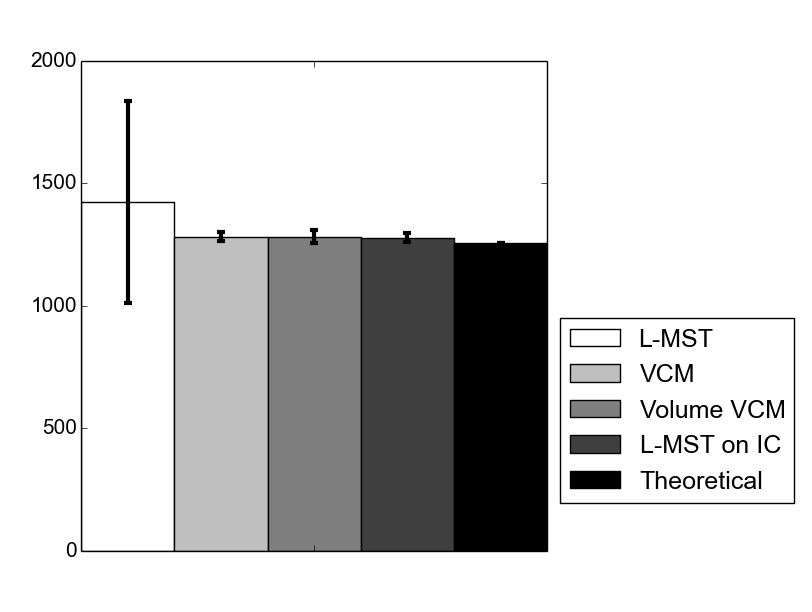
\includegraphics[width=0.8\textwidth, clip, trim = 0 1.5cm 6.6cm 0]{fig/corrected_area.png} %instead of noisy_area2.png
			\caption{Aire}
			\label{fig:areanoisy}
		\end{subfigure}%
		\begin{subfigure}[t]{0.5\textwidth}
			\centering
			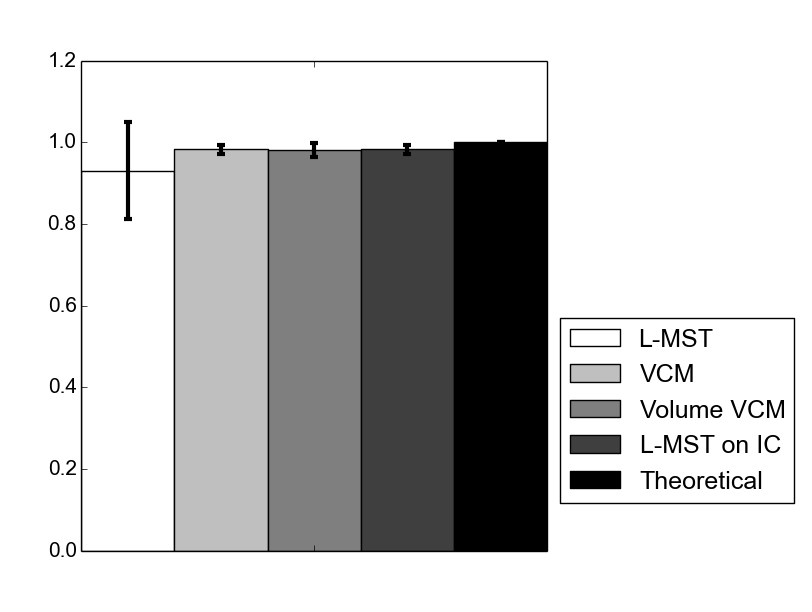
\includegraphics[width=1.2\textwidth, clip, trim = 0 1.5cm 0 0cm]{fig/corrected_round.png}
			\caption{Rotondité}
			\label{fig:roundnessnoisy}
		\end{subfigure}
	\end{figure}		
\end{frame}

\begin{frame}
	\frametitle{Volume synthétique (2)}
	\begin{itemize}
		\item Objet tubulaire avec variation de diamètre et d'ellipticité
		\item La normale du plan orthogonal est connue et la même en tout point du squelette
		\item Comparaison avec le plan calculé
	\end{itemize}
		\vspace{-0.3cm}
	\begin{figure}[h]
		\centering
		\begin{subfigure}[t]{0.5\textwidth}
			\centering
			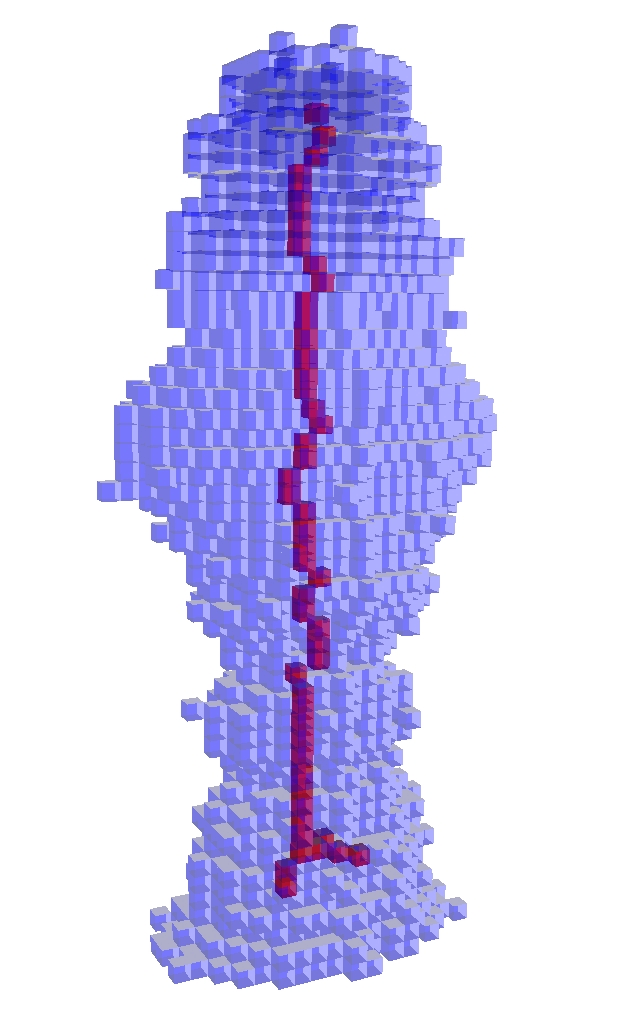
\includegraphics[scale=0.15, clip, trim=0 0 0 0]{fig/skeleton_and_cylinder.png}
			\label{fig:noisycylinder}
		\end{subfigure}%
		\begin{subfigure}[t]{0.5\textwidth}
			\centering
			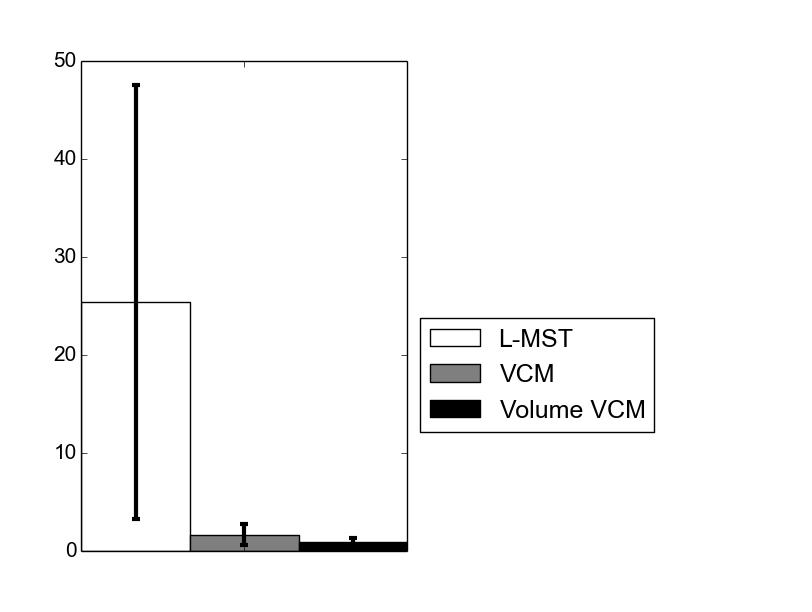
\includegraphics[width=1\textwidth, clip, trim=0.5cm 1cm 3cm 0.5cm]{fig/angle_defect.png}
			\label{fig:angledefect}
		\end{subfigure}
				
	\end{figure}
\end{frame}

\begin{frame}
	\frametitle{Données réelles}
	\begin{itemize}
		\item Volumes d'arbre bronchique issus d'acquisitions de scanner CT
		\item Comparaisons visuelles avec $\lambda$-MST
	\end{itemize}
		
	\begin{figure}[H]
		\begin{subfigure}[t]{0.5\textwidth}
			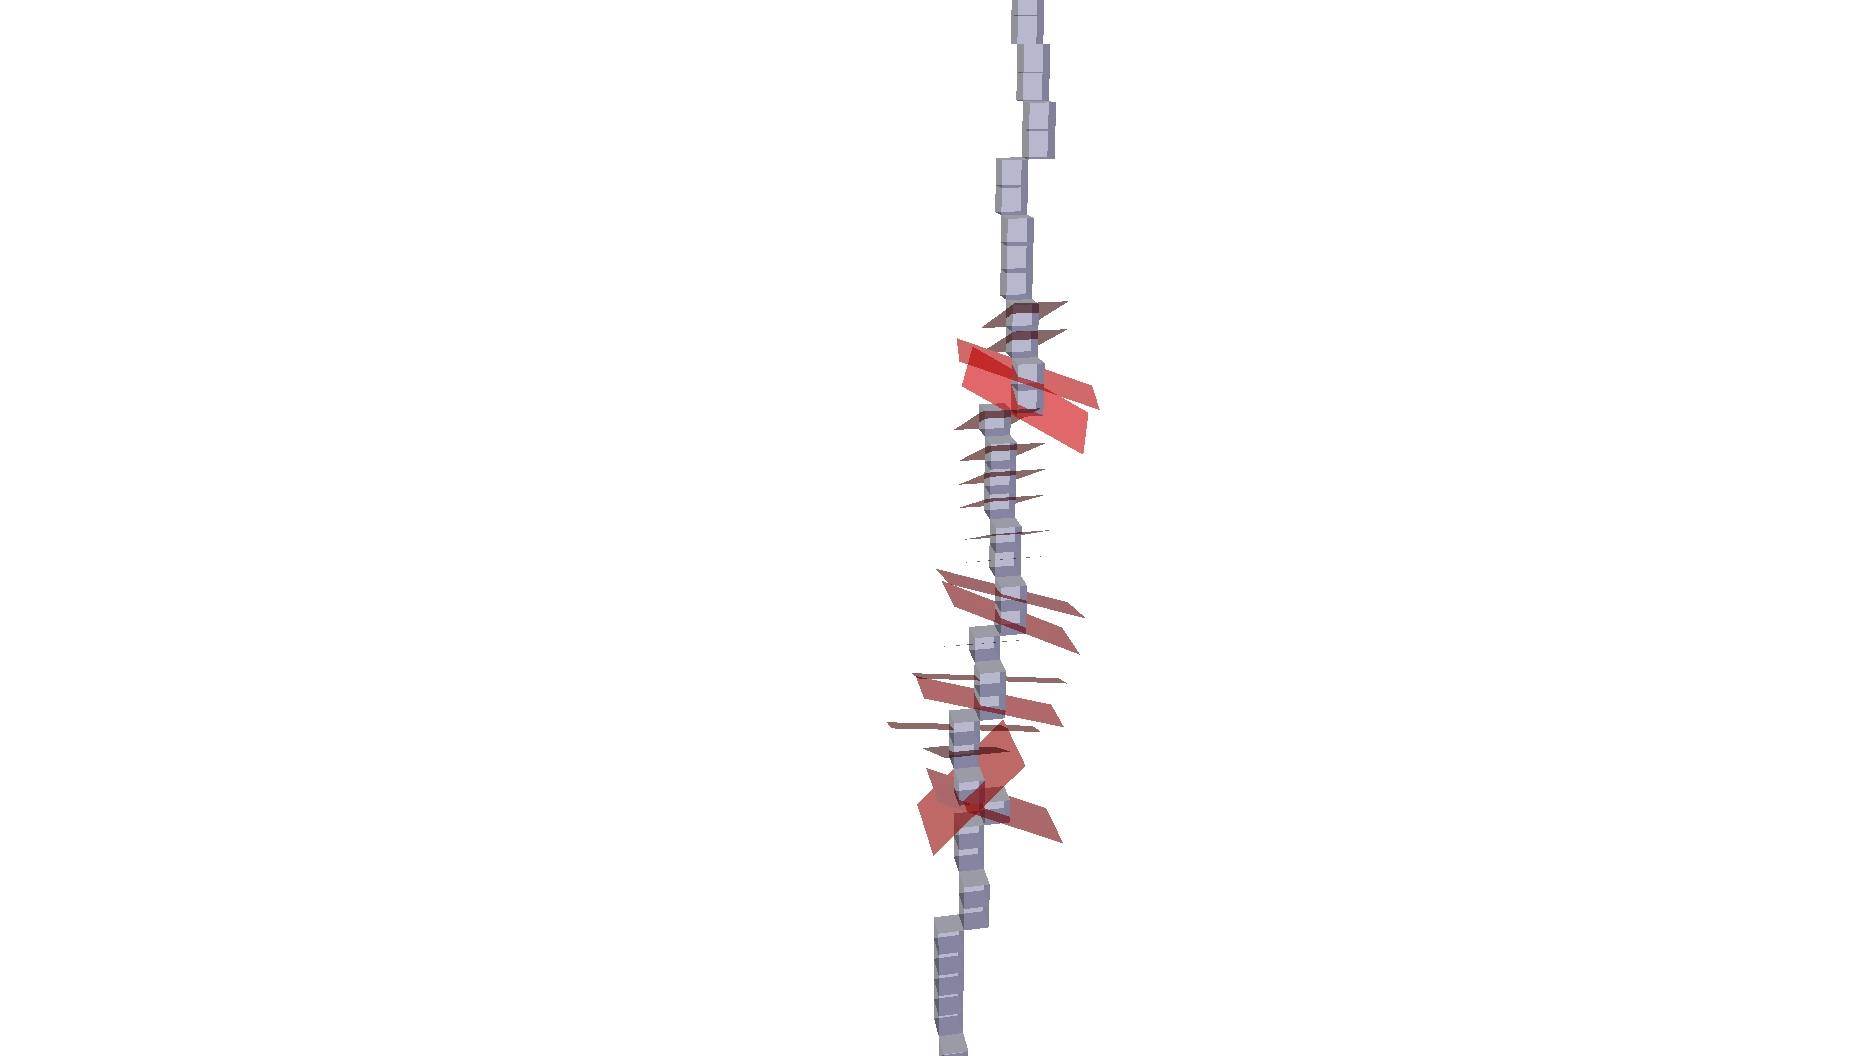
\includegraphics[angle=90, clip, trim=23cm 0cm 20cm 0, width=0.8\textwidth]{fig/mst_skeleton.png}
			\label{fig:mstskeleton}
		\end{subfigure}%
		\begin{subfigure}[t]{0.5\textwidth}
			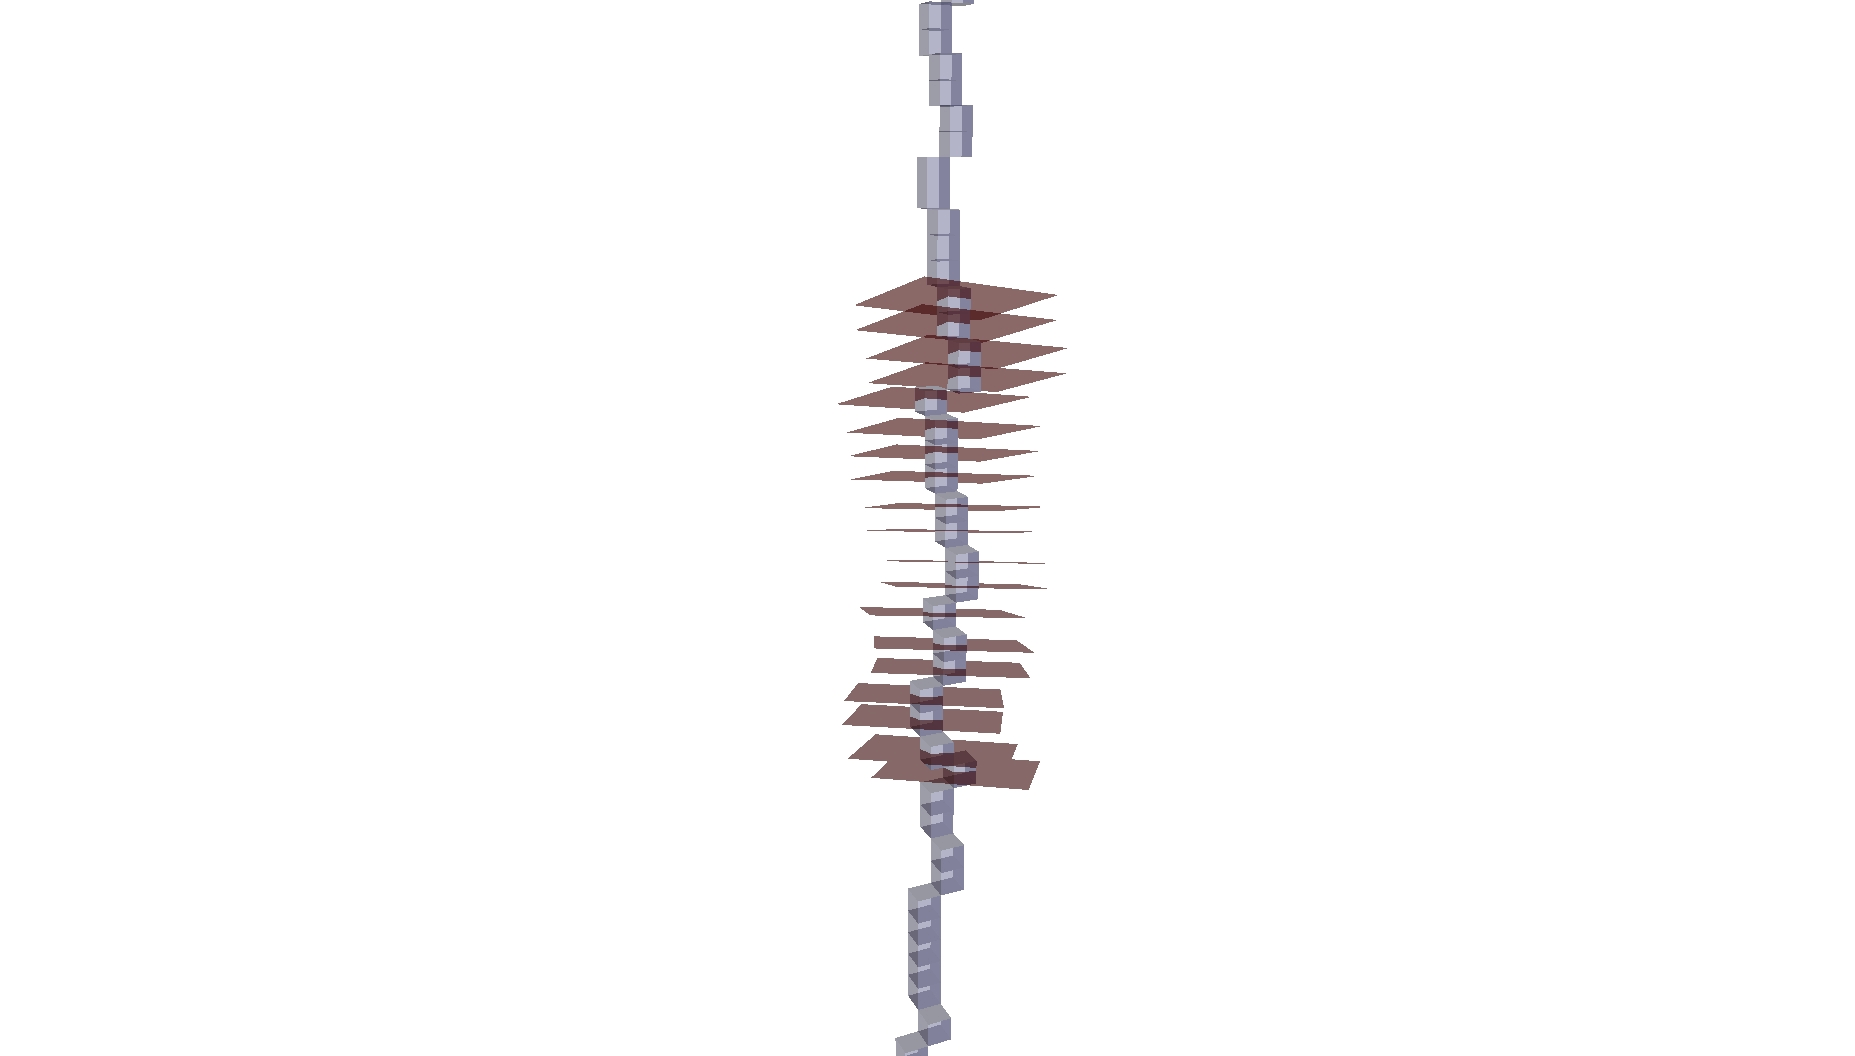
\includegraphics[angle=90,  clip, trim=23cm 0cm 20cm 0, width=0.8\textwidth]{fig/vcm_skeleton.png}
			\label{fig:vcmskeleton}
		\end{subfigure}
	\end{figure}
		
	\vspace{-0.5cm}
	\begin{figure}[H]
		\centering
		\begin{subfigure}[t]{0.5\textwidth}
			\centering
			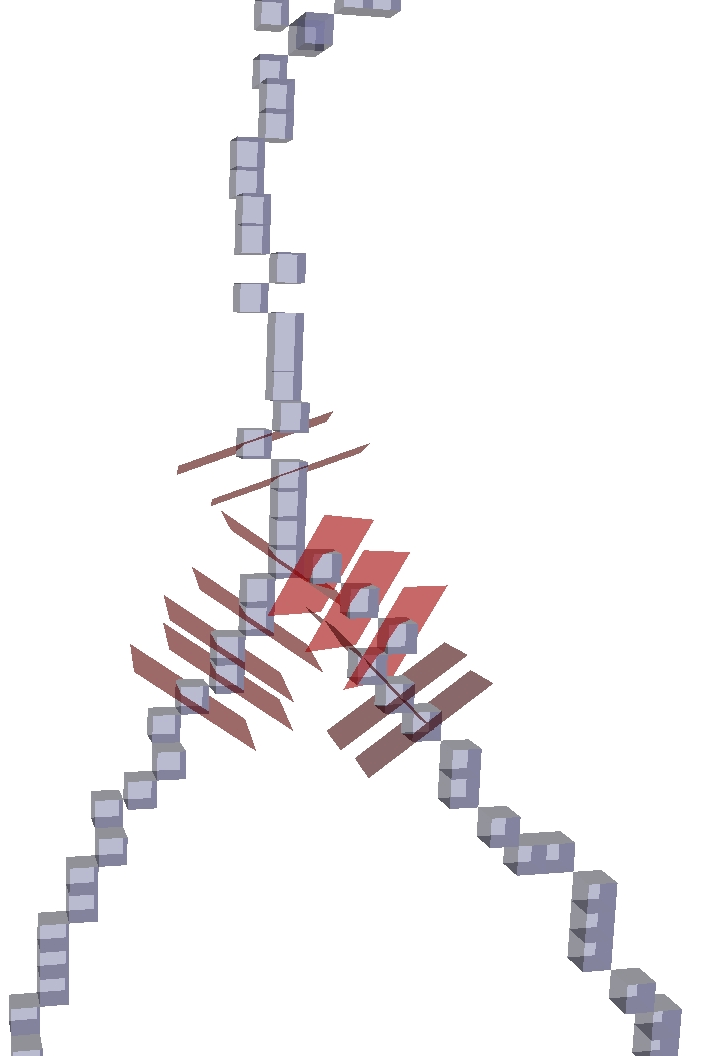
\includegraphics[clip, trim=0cm 0cm 0 0cm, width=0.4\textwidth]{fig/mst_branching.png}
			\caption{$\lambda$-MST}
		\end{subfigure}%
		\begin{subfigure}[t]{0.5\textwidth}
			\centering
			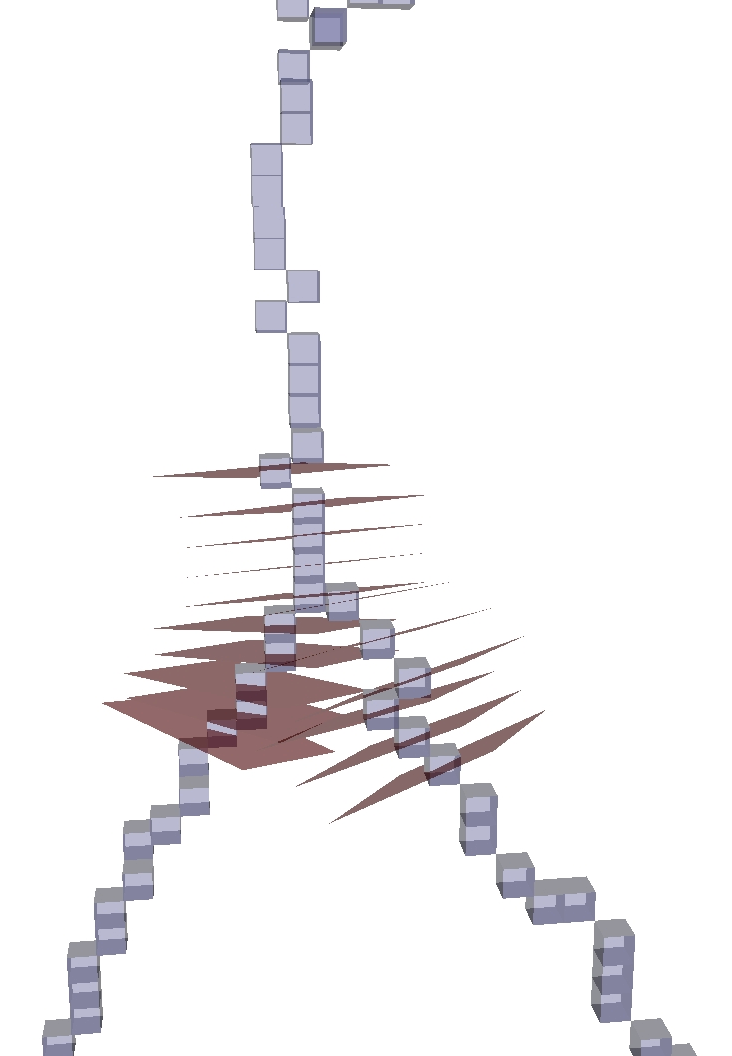
\includegraphics[clip, trim=0cm 0 0cm 3cm, width=0.4\textwidth]{fig/vcm_branching_3_15.png}
			\caption{VCM}
			\label{fig:vcmbranching}    
		\end{subfigure} 
	\end{figure}
\end{frame}


\section{Conclusion}
\begin{frame}
	\frametitle{Conclusion}
	\begin{block}{Résumé}
		\begin{itemize}
			\item Estimateur de plans orthogonaux sur des objets tubulaires
			\item Robuste aux perturbations sur les courbes discrètes
			\item Possibilité de s'abstraire du squelette
		\end{itemize}		
	\end{block}
	
	\begin{block}{Travaux en cours}
		\begin{itemize}
			\item Application sur les volumes: paramétrisation automatique
			\item Algorithme de squelettisation
		\end{itemize}
		
	\end{block}
\end{frame}

\begin{frame}
	\frametitle{Algorithme de squelettisation}
	\begin{itemize}
		\item Algorithme de suivi: déplacement avec la normale des plans orthogonaux
		\item Détection des jonctions: correspondent à des points de forte courbure $\Rightarrow$ détectés intrinsèquement par les VCM
				
		\item Soumis à DGCI 2016
	\end{itemize}
		
	\begin{columns}[onlytextwidth]
		\begin{column}{0.48\textwidth}
			\centering
			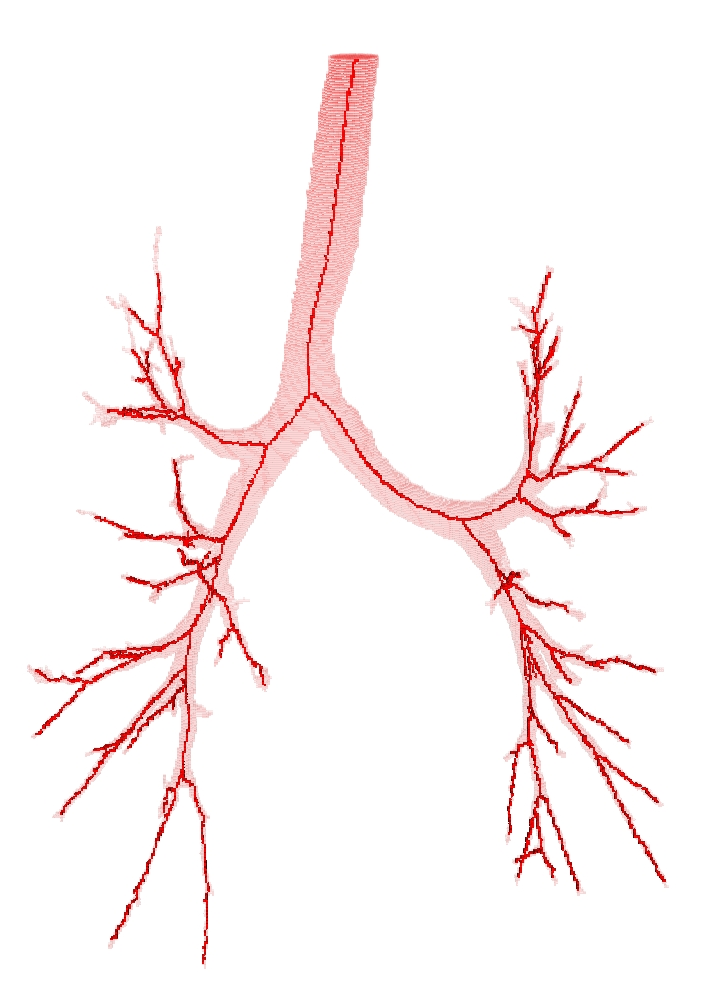
\includegraphics[width=0.6\textwidth]{fig/skeletonBronche2.png}
		\end{column}
					
		\begin{column}{0.48\textwidth}
			\centering
			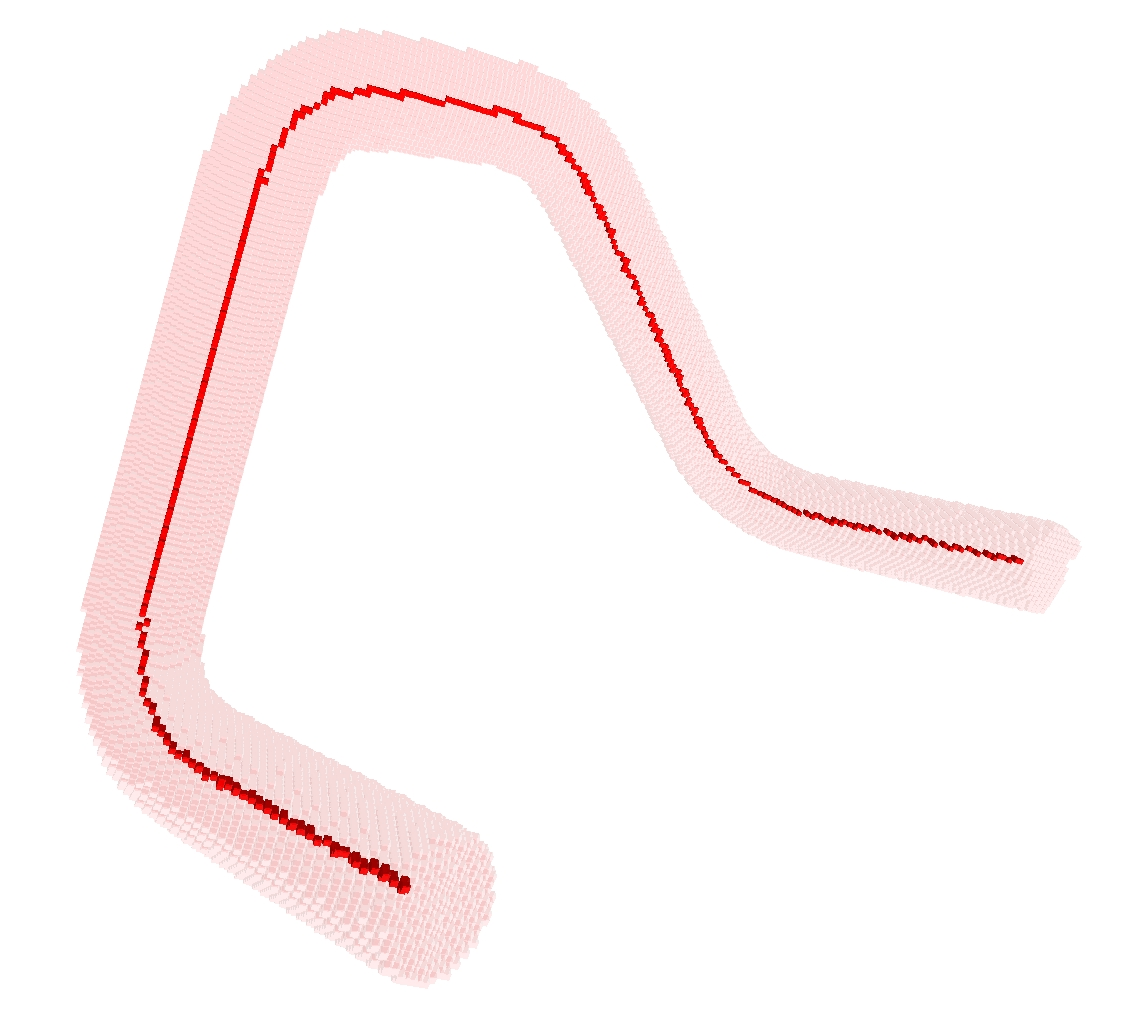
\includegraphics[width=0.7\textwidth]{fig/tubeBK.png}
		\end{column}		
	\end{columns}
			
			
\end{frame}


\logo{}
\plain{Merci de votre attention}

\end{document}
